\documentclass[a4paper, 12pt]{article}%тип документа

%отступы
\usepackage[left=2cm,right=2cm,top=2cm,bottom=3cm,bindingoffset=0cm]{geometry}

%Русский язык
\usepackage[T2A]{fontenc} %кодировка
\usepackage[utf8]{inputenc} %кодировка исходного кода
\usepackage[english,russian]{babel} %локализация и переносы

%Вставка картинок
\usepackage{wrapfig}
\usepackage{graphicx}
\graphicspath{{pictures/}}
\DeclareGraphicsExtensions{.pdf,.png,.jpg}

%оглавление
\usepackage{titlesec}
\titlespacing{\chapter}{0pt}{-30pt}{12pt}
\titlespacing{\section}{\parindent}{5mm}{5mm}
\titlespacing{\subsection}{\parindent}{5mm}{5mm}
\usepackage{setspace}

%Графики
\usepackage{multirow}
\usepackage{pgfplots}
\pgfplotsset{compat=1.9}

%Математика
\usepackage{amsmath, amsfonts, amssymb, amsthm, mathtools}

%Заголовок
\usepackage{lastpage} 
\usepackage{fancybox,fancyhdr}
\fancyhead[R]{\textit{Определение ширины запрещенной зоны полупроводника}}
\fancyhead[L]{\textit{Работа 11.1}}
\fancyhead[C]{}

\newtheorem{task}{Задача}
\begin{document}
		\begin{titlepage}
			\begin{center}
				\textit{Федеральное государственное автономное образовательное\\ учреждение высшего образования }
				\vspace{0.5ex}
				
				\textbf{«Московский физико-технический институт\\ (национальный исследовательский университет)»}
			\end{center}
			\vspace{10ex}
			\begin{center}
				\vspace{13ex}
				\textbf{Лабораторная работа № 11.1}
				\vspace{1ex}
				
				по курсу основы современной физики
				
				
				на тему:
				
				\textbf{\large{Определение ширины запрещенной зоны полупроводника}}
				
				\vspace{30ex}
				\begin{flushright}
					\noindent
					\textit{Работу выполнил:}
					\\
					\textit{Валеев Рауф
					}						 
				\end{flushright}
				\vfill
				Долгопрудный \\2021 год
			\end{center}
		\end{titlepage}
	
				\newpage	

	\pagestyle{fancy}
	
\textbf{Цель работы}: Исследуется температурная зависимость проводимости типичного полупроводника – германия или кремния. Определяется ширина запрещенной зоны полупроводника из полученной зависимости.

\section{Теоретическая справка}
Проводимость в полупроводниках зависит от количества электронов в зоне проводимости и дырок в валентной зоне.

Вероятность заполнения $f(\varepsilon)$ энергетических уровней электронами определяется функцией Ферми:
$$
f(\varepsilon) = \frac{1}{1+\exp\left(\frac{\varepsilon - \mu}{kT}\right)},
$$
где $\varepsilon$ -- значение энергии уровня в зоне проводимости, $\mu$ -- уровень Ферми. В приближении $(\varepsilon-\mu)>>kT$ имеем:

$$
f(\varepsilon) \approx \exp \left( - \frac{\varepsilon - \mu}{kT} \right).
$$

При небольших температурах электроны занимают нижние уровни, то есть $\varepsilon \approx \varepsilon_{c}$, 
$\varepsilon_{c}$ -- энергия, соответствующая дну зоны проводимости. Тогда количество электронов $n_n$
равно:
$$
n_{n}=Q_{n} \cdot f(\varepsilon) \approx Q_{n} \exp \left(-\frac{\varepsilon_{c}-\mu}{k T}\right).
$$
Здесь $Q_n$ -- количество занятых электронами уровней.
Вероятность возникновения дырки равна $1 - f(\varepsilon).$ В рассматриваемом приближении энергию дырок будем считать равной энергии верхней границы валентной зоны $\varepsilon$, тогда число дырок $n_p$ в валентной зоне определяется аналогично
$$
n_{p}=Q_{p} \cdot (1-f(\varepsilon)) \approx Q_{p} \exp \left(\frac{\varepsilon_{v}-\mu}{k T}\right).
$$
В чистых полупроводниках $n_n \approx n_p$, следовательно верно:
$$
n_{n} n_{p}=n^{2}=Q_{n} Q_{p} \exp \left(-\frac{\varepsilon_{c}-\varepsilon_{v}}{k T}\right).
$$
Ширину запрещенной зоны обозначим $\Delta=\varepsilon_{c}-\varepsilon_{v}$, тогда получим:
$$
n \propto \exp \left(-\frac{\Delta}{2 k T}\right).
$$
В присутствии электрического поля $Е$ средняя скорость $v$ носителя заряда
пропорциональна eмy: $v \propto E$.
Плотность тока в случае полупроводника запишется так: $$ j=j_n+j_p=|e|\left(n_n v_n+n_p v_p\right) \propto nE, $$ где
индексы $n$ и $p$ соответствуют электронам и дьркам. Из полученной пропорциональности
следует температурная зависимость проводимости полупроводника:
$$
\sigma_{s} \propto \exp \left(-\frac{\Delta}{2 k T}\right)
$$
\newpage

\section{Экспериментальная установка}
Для изучения зависимости $\sigma(T)$ используется установка, схематически изображенная на рис. $2 .$

Исследуемые образцы $\left(O_{1}\right.$ и $\left.O_{2}\right)$ в специальном зажиме помещаются в электронагревательную печь П. Сопротивление образцов измеряется универсальным цифровым вольтметром В7-34A, который обеспечивает

\begin{figure}[h]
\begin{center}
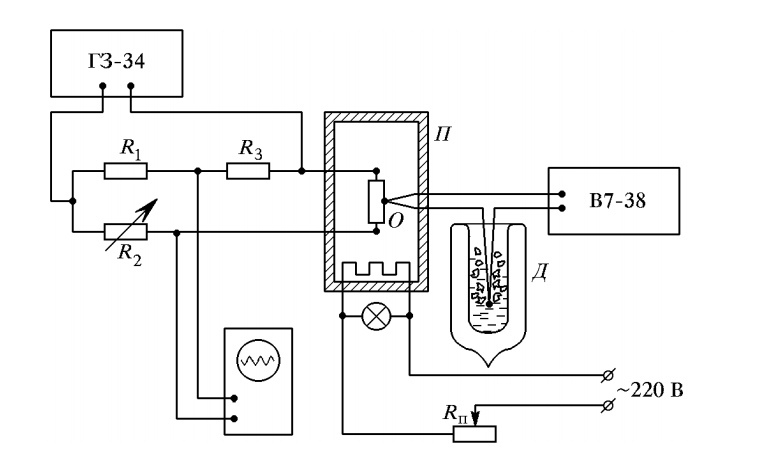
\includegraphics[scale=0.6]{5}
\end{center}
\caption{Экспериментальная установка}
\end{figure}

высокую точность измерений. В режиме измерения сопротивления на пределах 1 кОм, 10 кОм и 100 кОм погрешность в процентах не превышает
$$
\pm\left[0,015 \pm 0,02\left(R_{k} / R_{x}-1\right)\right]
$$
где $R_{k}-$ включенный предел измерений, $R_{x}$ - значение измеряемой величины в килоомах.

При этом ток через подключенный образец не превышает 1 мА. Поочередное подключение образцов к прибору осуществляется с помощью ключа $K .$ Один из образцов изготовлен из кристаллического германия (или кремния) и имеет форму прямоугольного параллелепипеда, другой - из тонкой медной проволоки длиной около двадцати MeTpOB. Удельная проводимость образцов находится по формуле
$$
\sigma=\frac{l}{R S}
$$
где $R-$ сопротивление образца, $l-$ его длина, $S-$ поперечное сечение образца. Размер образцов указан на установке.
\section{Измерения. Анализ результатов}
Результаты измерений занесем в таблицу: 

\begin{table}[h]
\begin{tabular}{|c|c|c|c|c|c|c|c|c|}
\hline
$U$, мВ & $T$, C & $T$, K & $1/T$, $10^{-3}$K & $R$, Ом & $\sigma$, $\frac{10^7}{\text{Ом} \cdot   \text{м}}$ & $\delta_{\sigma}$, $\frac{10^7}{\text{Ом}   \cdot \text{м}}$ & $\ln\left(\frac{\sigma}{\sigma_0}\right)$,   $\frac{1}{\text{Ом} \cdot \text{м}}$ & $\delta_{\ln\left(\frac{\sigma}{\sigma_0}\right)}$ \\ \hline
0,19    & 22     & 295,14 & 3,3882            & 62,2    & 5,6                                                 & 0,01                                                         & 0                                                                                 & 0,004                                              \\ \hline
0,52    & 30     & 303,14 & 3,2988            & 64,2    & 5,42                                                & 0,01                                                         & -0,033                                                                            & 0,004                                              \\ \hline
0,93    & 40     & 313,14 & 3,1935            & 66,5    & 5,24                                                & 0,01                                                         & -0,066                                                                            & 0,004                                              \\ \hline
1,36    & 50     & 323,14 & 3,0946            & 67      & 5,2                                                 & 0,01                                                         & -0,074                                                                            & 0,004                                              \\ \hline
1,79    & 60     & 333,14 & 3,0017            & 71,5    & 4,87                                                & 0,01                                                         & -0,14                                                                             & 0,004                                              \\ \hline
2,23    & 70     & 343,14 & 2,9143            & 74,3    & 4,69                                                & 0,01                                                         & -0,177                                                                            & 0,004                                              \\ \hline
2,68    & 80     & 353,14 & 2,8317            & 76,5    & 4,55                                                & 0,01                                                         & -0,208                                                                            & 0,004                                              \\ \hline
3,13    & 90     & 363,14 & 2,7538            & 78,7    & 4,42                                                & 0,01                                                         & -0,237                                                                            & 0,004                                              \\ \hline
\multicolumn{9}{|c|}{$\delta_T = 0,02 K$,   $\delta_{1/T} = 0,0002 K^{-1}$, $\delta_R = 0,1$ Ом, $\delta_U = 0,01$ мВ}                                                                                                                                                                                                \\ \hline
$U$, мВ & $T$, C & $T$, K & $1/T$, $10^{-3}$K & $R$, Ом & $\sigma$, $\frac{1}{\text{Ом} \cdot \text{м}}$      & $\delta_{\sigma}$, $\frac{1}{\text{Ом} \cdot \text{м}}$      & $\ln\left(\frac{\sigma}{\sigma_0}\right)$                                         & $\delta_{\ln\left(\frac{\sigma}{\sigma_0}\right)}$ \\ \hline
0,19    & 22     & 295,14 & 3,3882            &         &                                                     &                                                              &                                                                                   &                                                    \\ \hline
0,52    & 30     & 303,14 & 3,2988            & 708     & 3,294                                               & 0,005                                                        & 0                                                                                 & 0,003                                              \\ \hline
0,93    & 40     & 313,14 & 3,1935            & 441     & 5,288                                               & 0,012                                                        & 0,473                                                                             & 0,004                                              \\ \hline
1,36    & 50     & 323,14 & 3,0946            & 283     & 8,24                                                & 0,03                                                         & 0,917                                                                             & 0,005                                              \\ \hline
1,79    & 60     & 333,14 & 3,0017            & 188     & 12,4                                                & 0,07                                                         & 1,326                                                                             & 0,007                                              \\ \hline
2,23    & 70     & 343,14 & 2,9143            & 127     & 18,4                                                & 0,1                                                          & 1,72                                                                              & 0,007                                              \\ \hline
2,68    & 80     & 353,14 & 2,8317            & 72      & 32,4                                                & 0,5                                                          & 2,286                                                                             & 0,017                                              \\ \hline
3,13    & 90     & 363,14 & 2,7538            & 63      & 37                                                  & 0,6                                                          & 2,419                                                                             & 0,018                                              \\ \hline
\multicolumn{9}{|c|}{$\delta_T = 0,02 K$,   $\delta_{1/T} = 0,0002 K^{-1}$, $\delta_R = 1$ Ом, $\delta_U = 0,01$ мВ}                                                                                                                                                                                                  \\ \hline
\end{tabular}
\end{table}

Температуру получаем из напряжения по градуировочной таблице термопары. Все погрешности получаем из формулы метода наименьших квадратов.
\begin{figure}[h]
 \begin{center}
 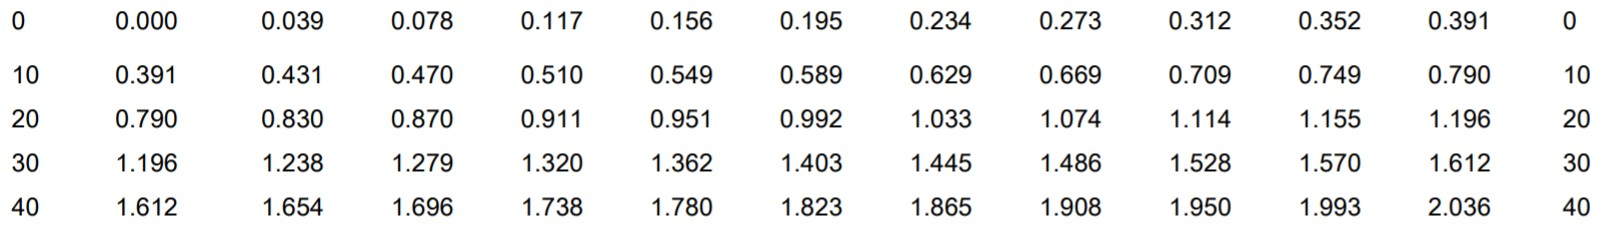
\includegraphics[width = \textwidth]{6}
 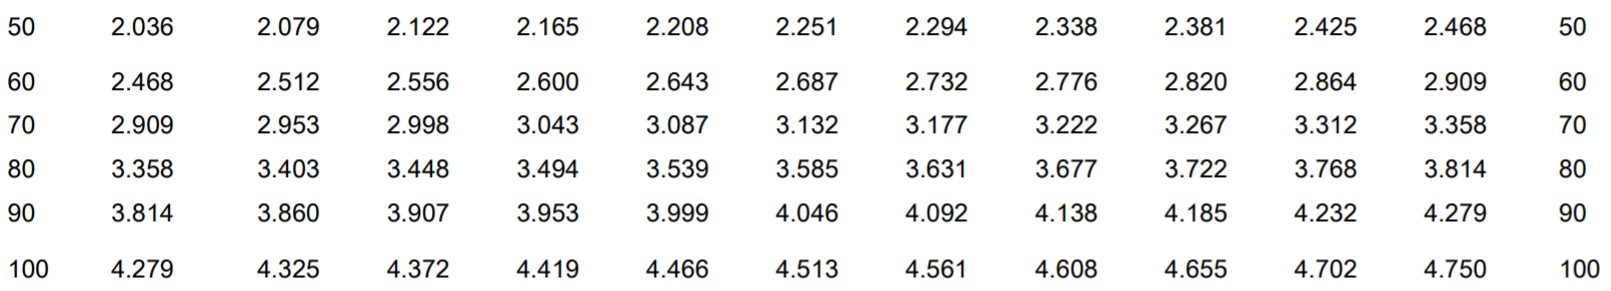
\includegraphics[width = \textwidth]{7}
 \caption{Градуировочная таблица медь-константановой термопары}
 \end{center}
 \end{figure} 
\newpage
Построим графики зависимости $\sigma_x(T)$ и $\ln(\sigma/\sigma_0) \text{ от } 1/T$ для обоих образцов.
\begin{figure}[h]
\begin{center}
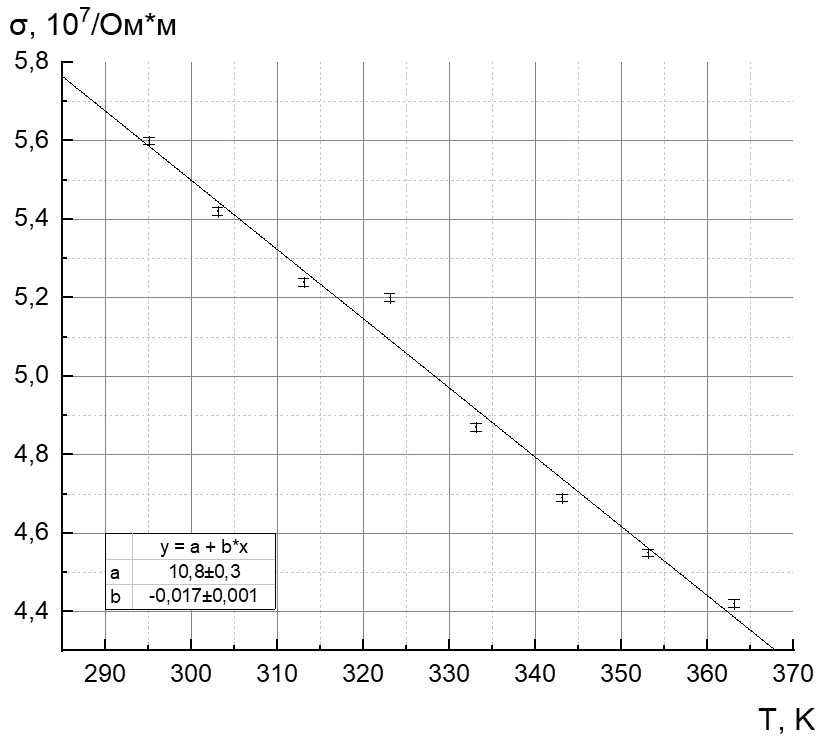
\includegraphics[width = \textwidth]{1}
\caption{График зависимости $\sigma$ от $T$ для меди}
\end{center}
\end{figure}
Определим по наклону графика $\sigma(T)$ температурный коэффициент сопротивления:

Для меди мы получили, что 
\[\sigma = a + b \cdot T\]

Получаем, что если мы поделим $b$ на $a$, то мы получим искомую величину:
\[\alpha = \frac{a}{b}\]
\[\sigma_{\alpha} = \alpha \cdot \sqrt{\left(\frac{\sigma_a}{a}\right)^2 + \left(\frac{\sigma_b}{b}\right)^2}\]
В итоге получаем, что 
\[\alpha = -0,0016 \pm 0,0001 K^{-1}\]
В таблице указаны данные в градусах Цельсия, для этого нужно пересчитать коэффицент для градуировки температуры в цельсиях: $a' = a + b \cdot 273,15 K \approx 4,5 \Rightarrow \alpha = 0,0038 C^{-1}$ а уже это число соответствует теоретическому $\alpha_{th} = 0,004 C^{-1}$, что означает, что наше полученное значение совпадает с табличным.

\begin{figure}[h]
\begin{center}
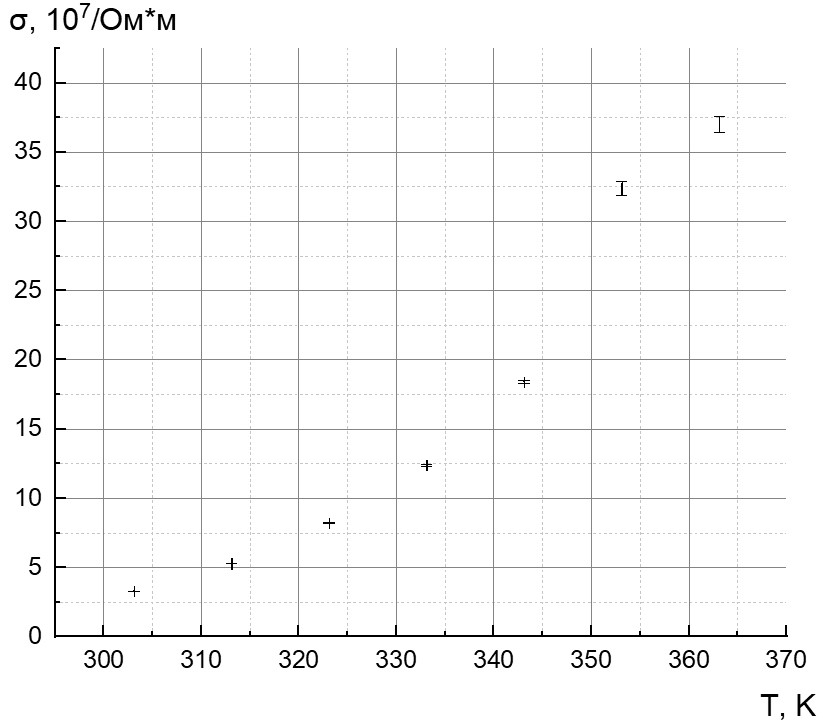
\includegraphics[width = \textwidth]{3}
\caption{График зависимости $\sigma$ от $T$ для полупроводника}
\end{center}
\end{figure}

Как видно из графиков, $\sigma$ для меди падает линейно, когда как для полупроводника она растет. Это связано с тем, что для металла все электроны свободные, и у них линейно увеличивается подвижность электронов, когда как для полупроводника ключевую роль играет попадание электрона в зону проводимости, которая зависит от экспоненты, из-за чего и получаем такие зависимости.
\newpage
\begin{figure}[h]
\begin{center}
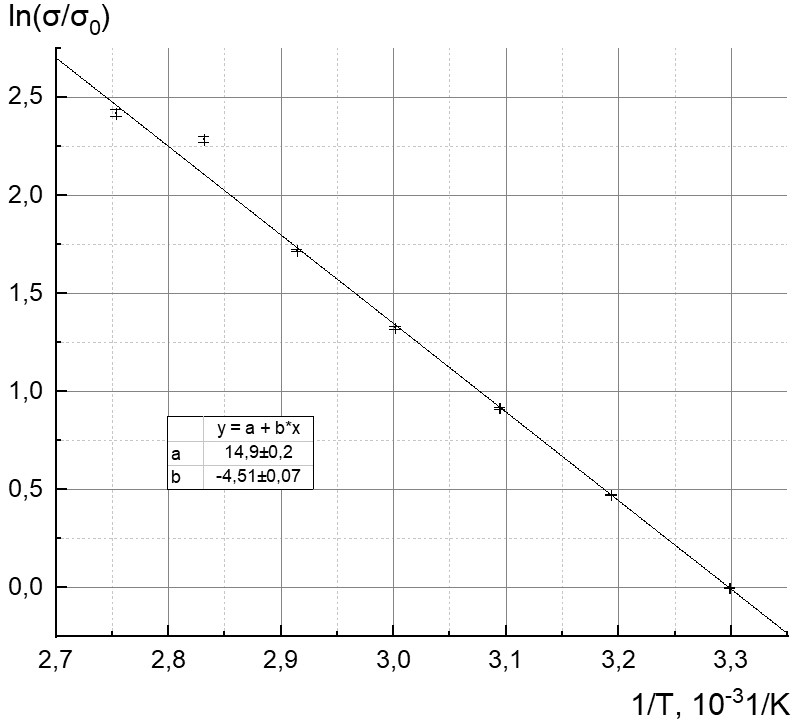
\includegraphics[width = \textwidth]{4}
\caption{График зависимости $\ln\left(\frac{\sigma}{\sigma_0}\right)$ от $1/T$ для полупроводника}
\end{center}
\end{figure}

Теперь определим ширину запрещенной зоны для графика зависимости логарифма $\sigma$ от $1/T$. 

Получаем искомую $\Delta$ из формулы 
\[\sigma \approx = A \exp\left(-\frac{\Delta}{2 k_B T}\right)\]

В итоге получаем, что коэффициент наклона графика будет равен $\frac{\Delta}{2 k_B}$
То есть 
\[\Delta = -2 k_B \cdot b = \left(12,4 \pm 0,2\right) \cdot 10^{-20} \text{Дж} = 0,774 \pm 0,012 \text{эВ}\]

\[\Delta_{Ge} = 0,75 \text{эВ}\]
Это означает, что мы получили искомое значение, приближенное к теории.

\section{Вывод}
В ходе работы мы исследовали характер поведения проводимости от температуры и получили, что и ожидалось: электропроводность линейно убывает с ростом температуры для проводника и экспоненциально растет для полупроводника. Так же мы посчитали тепловой коэффициент теплопроводности, который совпадает с табличным, как и ширина запрещенной зоны, которая оказалось довольно точной, поскольку у нас в качестве полупроводника был использован Германий.
\begin{thebibliography}{3}
\bibitem{I_2}
Игошин Ф. Ф., Самарский Ю. А., Ципенюк Ю. М. Лабораторный практикум по общей физике: квантовая физика. МФТИ, 2012.
\end{thebibliography}
\end{document}